%!TEX root = ../main.tex
%%%%%%%%%%%%%%%%%%%%%%%%%%%%%%%%%%
% Links:
%
% Difficulty:
% Companies: 
%%%%%%%%%%%%%%%%%%%%%%%%%%%%%%%%%%

\chapter{Tree Diameter}
\label{ch:tree_diameter}
\section*{Introduction}
The problem described in this chapter is quite simple and can be solved very elegantly and very quickly considering it can be coded in an handful of lines. Therefore it is really important we understand all the pieces that make up the solution for this one so we will be able to sort this out fast during an interivew.

\section{Problem statement}
\begin{exercise}
 Given a binary tree, you need to compute the length of the diameter of the tree. The diameter of a binary tree is the length of the longest path between any two nodes in a tree.

 The length of path between two nodes is represented by the number of edges between them.

 The definition of the tree is shown in Listing \ref{list:verify_BST:tree_structure}.


	\begin{example}
	\hfill \\
	Given the binary tree shown in Figure \ref{fig:tree_diameter:example1} the function return $3$. One path of such length is from node $4$ (or $5$) to node $3$.
	\end{example}

\end{exercise}

\begin{figure}
	\centering
	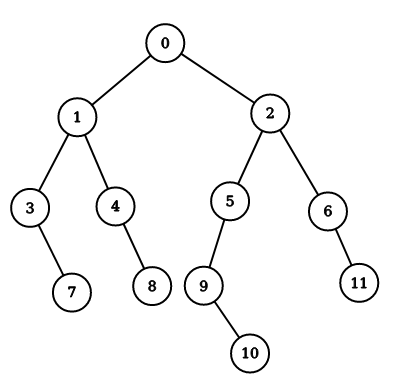
\includegraphics[scale=0.4]{sources/tree_diameter/images/example1}
	\caption{Visual representation of the example $1$ of the problem calculating the tree of a diameter.}
	\label{fig:tree_diameter:example1}
\end{figure}


\section{Clarification Questions}

\begin{QandA}
	\item 
	\begin{answered}
		\textit{}
	\end{answered}
	
\end{QandA}

\section{Discussion}
\label{tree_diameter:sec:discussion}


\subsection{Brute-force}
\label{tree_diameter:sec:bruteforce}

\lstinputlisting[language=c++, caption={Sample Caption},label=list:tree_diameter]{sources/tree_diameter/tree_diameter_solution1.cpp}

